\documentclass[a4paper]{article}
\usepackage[utf8]{inputenc}
\usepackage[russian]{babel}
\usepackage[T2]{fontenc}
\usepackage[warn]{mathtext}
\usepackage{graphicx}
\usepackage{amsmath}
\usepackage{floatflt}
\usepackage[left=20mm, top=20mm, right=20mm, bottom=20mm, footskip=10mm]{geometry}


\graphicspath{ {images/} }
\usepackage{multicol}
\setlength{\columnsep}{2cm}


\begin{document}

\begin{titlepage}
	\centering
	\vspace{5cm}
	{\scshape\LARGE Московский физико-технический институт \par}
	\vspace{5cm}

	{\huge\bfseries Термоэлектронный диод \par}
	\vspace{1cm}
	{\scshape\Large Лабораторная работа по курсу <<Вакуумная электроника>>\par}
	\vspace{1cm}
	\vfill
\begin{flushright}
	{\large выполнила студентка 004 группы ФЭФМ}\par
	\vspace{0.3cm}
	{\LARGE Плюскова Наталия Алексеевна} \par

	
\end{flushright}
	

	\vfill

% Bottom of the page
	Долгопрудный, 2021 г.
\end{titlepage}

\section{Цель работы}
\begin{enumerate}
    \item Изучить физические принципы электроконтактной сварки
    \item Овладеть основными приёмами различных сварочных операций
\end{enumerate}

\section{Виды электроконтактной сварки}
{\it Электроконтактная сварка} - комплексный электромеханический процесс, при котором нагрев места соединения производится проходящим через него электрическим током и сопровождается приложением усилий сжатия. \par 
Виды электроконтактной сварки:
\begin{itemize}
    \item {\it Точечная сварка} выполняется в виде отдельных точек с интервалом между ними. Одна из разновидностей точечной сварки - рельефная сварка.
    \item {\it Роликовая сварка} - при её выполнении соединение деталей производится с помощью вращающихся электродов-роликов. Роликовая сварка подразделяется на непрерывную (непрерывная подака тока в сварочную цепь и образование ряда точек, перекрывающих друг друга, в результате чего получается сплошной герметичный шов), и прерывистой (на ролики подаются кратковременные импульсы тока, соединения не отличаются от выполненных точечно)
    \item {\it Стыковая сварка} - электрический ток проходит через стык соединённых деталей, разогревая их концы, после чего прилагается усилие сжатия.
\end{itemize}

\begin{figure}[h]
    \centering
    \includegraphics[width=7.5 cm]{weld_types.png}
    \caption{Виды электроконтактной сварки: а) — точечная, б) — роликовая, в) — стыковая; 1, 2 — свариваемые детали; 3, 4 – электроды}
    \label{fig:vac}
\end{figure}

\section{Требования к сварочным соединениям}

При изготовлении электровакуумных приборов часто необходимо изготовление неразъёмных соединений деталей, выполненных из металлов с различными электрофизическими свойствами. Более 90\% всех сварных соединений в электровакуумной технике производится с помощью электроконтактной сварки.\par
Требования к таким соединениям:
\begin{enumerate}
    \item Высокая статическая и динамиеская прочность при длительной работе в вакууме и при других нагрузках
    \item Высокая электро- и теплопроводность
    \item Соответствие требованиям вакуумной чистоты (отсутствие шлаков, летучих соединений, других посторонних частиц)
\end{enumerate}

Качество соединений зависит от:
\begin{itemize}
    \item Предварительной подготовки поверхности деталей (полировка, обезжиривание)
    \item Усилия сжатия
    \item Сварочного тока
    \item Времени сварки.
\end{itemize}

\section{Принципы работы сварочного оборудования}
По способу получения сварочного тока электроконтактная сварка разделяется на трансформаторную и импульсную. \par
{\it Трансформаторная сварка} используется в случаях, когда приходится производить сварку в сильно различающихся режимах и высокая производительность не важна. Усилие сжатия и время прохождения тока определяются сварщиком, поэтому качество сварки напрямую зависит от его квалификации. Трансформаторная сварка не позволяет работать в режиме, требующем короткого времени сварки. \par 
{\it Импульсная сварка} используется для режимов, требующих короткого времени сварки. Формирование импульса напряжения проиходит только после достижения требуемого механического усилия на детали. Импульсные формирователи обычно выполняют по {\it тиристорной} или {\it конденсаторной} схемам. Детали во время сварки могут удерживаться как вручную, так и при помощи специальных оправок. Для повышения производительности и повторяемости сварочного процесса могут быть использованы автоматические установки с возможностью задания на них усилия сжатия, длительности и мощности сварочного импульса.  

\section{Лабораторная установка}
Схема лабораторной установки для исследования характеристик термоэлектронного диода приведена на рис. 1.

\begin{figure}[h]
    \centering
    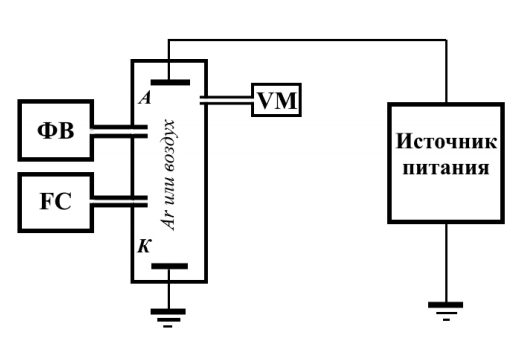
\includegraphics[width=13cm]{setup.PNG}
    \caption{Принципиальная схема лабораторной установки}
    \label{fig:vac}
\end{figure}
\begin{enumerate}
    \item Форвакуумный насос
\item Турбомолекулярный насос
\item Вакуумная камера
\item Клапан с электрическим управлением
\item Измерительная насадка
\item Фильтр входящего воздуха
\item Диод
\item Источник питания HY 3010E
\item Вольтметр GPR-30H100
\end{enumerate}

\section{Изготовление диода}
\subsection{Изготовление анода}
\begin{itemize}
    \item Для изготовления анода используем никелевую пластину $30 \cdot 40~\text{мм}$. Для большей жесткости анода на заготовке с помощью шила проводятся канавки (ребра жесткости).
    \item Заготовка наматывается на оправку с захлестом $3~\text{мм}$, а края пластины завальцовываются на шве для более плотного прилегания.
    \item Сварка производится с шагом $3~\text{мм}$ межу точками.
\begin{figure}[h]
\begin{center}
\includegraphics[width=13cm]{заготовка анода.jpg}
\end{center}
\end{figure}
\end{itemize}
\subsection{Монтаж анода на ножку}
\begin{itemize}
    \item Изготавливаем траверсы из двух отрезков никелевой проволоки по $50~\text{мм}$ каждый. Проволока прокатывается между двух пластин для выравнивания и профилируется.
    \item Траверсы привариваются к аноду так, чтобы ось анода находилась строго между ними.
\begin{figure}[h]
\begin{center}
\includegraphics[width=13cm]{траверса анода.jpg}
\end{center}
\end{figure}
    \item Далее анод монтируется на ножу так, как показано на рисунке ниже. Предварительно надо очистить выводы ножки от окисла при помощи надфиля.
\end{itemize}
\begin{figure}[h]
\begin{center}
\includegraphics[width=13cm]{посадка на ножку.jpg}
\end{center}
\end{figure}
\newpage
\subsection{Подготовка крепления катода}
\begin{itemize}
    \item Для изготовления катода необходимы никелевая проволока длиной $80~\text{мм}$ и две полоски из никела размерами $2 \cdot 20~\text{мм}$ и  $2 \cdot 10~\text{мм}$. Для изготовления самого катода понадобится отрезок вольфрамовой проволоки длиной $50~\text{мм}$.
    \item Сначала изготавливается траверса и два крепления катода, затем на конец натягивающей траверсы приваривается первое крепление и сама траверса приваривается на соответствующий вывод ножки (см. рисунок)
\begin{figure}[h]
\begin{center}
\includegraphics[width=13cm]{натягивающая траверса катода.jpg}
\end{center}
\end{figure}
\end{itemize}
\subsection{Монтаж катода}
\begin{itemize}
    \item Сначала отрезок вольфрамовой проволоки распрямляется, затем катод закрепляется во втором креплении.
\begin{figure}[h]
\begin{center}
\includegraphics[width=13cm]{заварка катода.jpg}
\end{center}
\end{figure}
    \item Далее крепление вместе с катодом приваривается на соответствующий вывод ножки.
    \item Происходит натягивание и фиксация катода: для этого свободный конец катода вкладывается в согнутое крепление на натягивающей траверсе. Затем катод натягивается и его приваривают к креплению.
\end{itemize}

\newpage
\section{Выполнение работы}
\begin{enumerate}
    \item Сначала проведём прогрев катода, снимем зависимость тока накала от напряжения накала. График зависимости приведён на рисунке 2.

\begin{figure}[h]
\begin{center}
\includegraphics[width=13cm]{fig1.png}
\caption{Зависимость тока накала от напряжения накала}
\end{center}
\end{figure}
   
\item Рассчитаем сопротивление диода по формуле, нанесем погрешности на график:
\begin{center}
    $R = \frac{U}{I}$,
\end{center}
$$\sigma_R = \sqrt{(\sigma_U / I)^2 +(\sigma_I U/I^2)^2}$$
Рассчитаем подаваемую мощность, нанесём погрешности на график:
\begin{center}
    $P = U I$
\end{center}
$$\sigma_P = \sqrt{(\sigma_U I)^2 +(\sigma_I U)^2}$$
Построим график зависимости сопротивления катода от приложенной мощности (рисунок 3)



\item Построим графики зависимости температуры катода от тока накала.  \par
Для графика, построенного на основании изменения сопротивления катода, температуру будем вычислять по формуле, полученной в результате преобразований:
\begin{center}
   $ R_T = R_0 (1 + \alpha T) $, \\
   $T = \frac{R_T - R_0 }{\alpha R_0}$
\end{center}
где $\alpha = 9,29 * 10^{-3}$ - коэффициент температурной зависимости электрического сопротивления, $\rho_0$ - удельное сопротивление материала катода при $0^{\circ}$. Учтем длину и диаметр проволоки. \par

Для графика, построенного на основании расчётов с использованием уравнения энергетического баланса, используем формулу 
\begin{center}
    $T_k = (\frac{P}{\varepsilon S \sigma})^{1/4}$,
\end{center}
где $S$ - площадь эмитирующей поверхности, $\varepsilon = 0.032$ - степень черноты материала катода, $\sigma = 5.67*10^{-8}$ Дж/(с*м$^2$*K$^4$). \par
Представим эти зависимости на одном графике (рисунок 4).




\item Построим графики зависимости анодного тока от анодного напряжения при различных значениях тока накала (рисунки 5 - 11). Покажем прямую линию, отвечающую аппроксимации начального участка графика уравнением вида $I_A = g (V_A)^{3/2}$



\item По этим данным определим первеанс диода $g$. Зная, что $I_a = gV_A^{3/2}$ и имея зависимости $\lg(I_A) = k \lg(V_A) + b$, получим
\begin{center}
    $g = 10^{\frac{3b}{2k}}$
\end{center}

Определим первеанс по разным данным тока накала диода и сравним значения с расчётным:

\begin{center}
    $g = 2.33*10^{-6} \frac{S_c}{R_a ^2} = 3.4485*10^{-3}$,
\end{center}
где $S_c$ - площадь поверхности катода, $R_a$ - радиус анода. \par

Также вычислим отношение заряда электрона к его массе по формуле

\begin{center}
   $e/m = \frac{81}{8}(g\frac{R_a}{L_a})^2$
\end{center}

Вычислим эффективность катода:
\begin{center}
    $\eta = \frac{I}{P}$
\end{center}

    \begin{table}[h]
    \centering
    \begin{center}
    \caption{Значения первеанса по разным опытам}
    \end{center}
    \vspace{0.1cm}
    \label{tab:my_label}
    \begin{tabular}{ |p{1cm}|p{1cm}|p{1cm}|p{2cm}|p{2cm}|p{2cm}|p{2cm}|}
 \hline
 $I$, А & $U$, B & k & b & g & e/m & $\eta$, \% \\
 \hline
2.4 & 4.7 & 0.137 & -4,4898 & 6.944*$10^{-50}$ & -- & 21.3\\
 \hline
2.5 & 5.3 & 0.2409 & -4,0071 & 1.12*$10^{-25}$ & 3.528*$10^{-51}$ & 18.7\\
 \hline
2.6 & 5.5 & 0.3184 & -3,7983 & 1.27*$10^{-18}$ & 4.536*$10^{-37}$ & 18.0\\
 \hline
2.7 & 6.0 & 0.5798 & -3,7735 & 1.73*$10^{-10}$ & 8.41*$10^{-21}$ & 16.7\\
 \hline
2.8 & 6.3 & 0.7506 & -3,7191 & 3.69*$10^{-8}$ & 3.83*$10^{-16}$ & 15.9 \\
 \hline
2.9 & 6.6 & 1.0087 & -3,8266 & 2.04*$10^{-6}$ & 1.17*$10^{-12}$ & 15.0\\
 \hline
3.0 & 7.0 & 1.2219 & -3,9186 & 1.55*$10^{-5}$ & 6.75*$10^{-11}$ & 14.3\\
 \hline 
\end{tabular}
\end{table}

\item Построим зависимость анодного тока от тока накала при напряжении V = 110 B

\end{enumerate}

\section{Вывод}

В ходе лабораторной работы
\begin{enumerate}
    \item Были изготовлен диод методом электроконтактной сварки
    
    \item Были получены представления о структуре элементарного диода

    \item Была исследована вольт-амперная характеристика диода
    
    \item Был рассчитан первеанс, эффективность и отношение заряда электрона к его массе

    \item Были проверены и подтверждены закономерности ВАХ диода: при больших токах накала - справедливо уравнение Чайлда-Ленгмюра, а при насыщении – уравнение Ричардсона-Дэшмана;

    \item Была рассчитана температура катода двумя разными способами: используя сопротивление катода, используя уравнение энергетического баланса, при помощи уравнения Ричардсона-Дэшмана построить зависимость T(I накала) не удалось, так как явной зависимости между T и I накала нет, а численные методы решения не дали результатов, схожих с двумя предыдущими графиками.
    
    \item Мы ознакомились с принципами работы сварочного оборудования, используемого в электровакуумном производстве, его основными характеристиками. Были изучены различные дефекты, возникающие при сварке, и причины их возникновения. При выполнении практической части были проведены простейшие сварочные операции (сварка пластина-пластина, пластина-проволока), изготовлены заготовка анода и траверсы.

\end{enumerate}

\section{Список литературы}
\begin{enumerate}
    \item Батурин А.С., Кириченко Л.А., Коновалов Н.Д. и др. Под ред. Шешина Е.П. Эмиссионная электроника в примерах и задачах: учебное пособие / --М.:МФТИ, 2002 - 193 с. 
    \item Батурин А.С., Стариков П.А., Шешин Е.П. Термоэлектронный диод: лабораторная работа по курсу Вакуумная электроника /--М.:МФТИ, 2008 - 43 с.
\end{enumerate}

\newpage


\begin{figure}[h]
\begin{center}
\includegraphics[scale=0.4]{fig2.png}
\caption{Зависимость сопротивления катода от приложенной мощности}
\end{center}
\end{figure}

\begin{figure}[h]
\begin{center}
\includegraphics[scale=0.4]{fig3.png}
\caption{Зависимость температуры катода от тока накала: расчёт по измерению сопротивления и по уравнению Стефана-Больцмана}
\end{center}
\end{figure}

\begin{figure}[h]
\begin{center}
\includegraphics[width=13cm]{2_4.png}
\caption{Зависимость $lg(I_A)$ от $lg(V_A)$ при токе накала 2.4 А, напряжении накала 4.7 B}
\end{center}
\end{figure}

\begin{figure}[h]
\begin{center}
\begin{minipage}[h]{0.45\linewidth}
\includegraphics[width=1\linewidth]{2_5.png}
\caption{Зависимость $lg(I_A)$ от $lg(V_A)$ при токе накала 2.5 А, напряжении накала 5.3 B}
\end{minipage}
\hfill 
\begin{minipage}[h]{0.45\linewidth}
\includegraphics[width=1\linewidth]{2_6.png}
\caption{Зависимость $lg(I_A)$ от $lg(V_A)$ при токе накала 2.6 А, напряжении накала 5.5 B }
\end{minipage}
\end{center}
\end{figure}

\begin{figure}[h]
\begin{center}
\begin{minipage}[h]{0.45\linewidth}
\includegraphics[width=1\linewidth]{2_7.png}
\caption{Зависимость $lg(I_A)$ от $lg(V_A)$ при токе накала 2.7 А, напряжении накала 6.0 B}
\end{minipage}
\hfill 
\begin{minipage}[h]{0.45\linewidth}
\includegraphics[width=1\linewidth]{2_8.png}
\caption{Зависимость $lg(I_A)$ от $lg(V_A)$ при токе накала 2.8 А, напряжении накала 6.3 B }
\end{minipage}
\end{center}
\end{figure}

\begin{figure}[h]
\begin{center}
\begin{minipage}[h]{0.45\linewidth}
\includegraphics[width=1\linewidth]{2_9.png}
\caption{Зависимость $lg(I_A)$ от $lg(V_A)$ при токе накала 2.9 А, напряжении накала 6.6 B}
\end{minipage}
\hfill 
\begin{minipage}[h]{0.45\linewidth}
\includegraphics[width=1\linewidth]{3_0.png}
\caption{Зависимость $lg(I_A)$ от $lg(V_A)$ при токе накала 3.0 А, напряжении накала 7.0 B }
\end{minipage}
\end{center}
\end{figure}

\begin{figure}[h]
\begin{center}
\includegraphics[width=13cm]{fig4.png}
\caption{Зависимость $lg(I_A)$ от тока накала при V = 140 B}
\end{center}
\end{figure}

\end{document}
